\chapter{Literature Review}

\section{Introduction}
This chapter reviews the existing literature and practice related to e-commerce platforms, web frameworks for custom online stores, applications of AI in e-commerce, and online payment integration with a focus on developing-country contexts such as Bangladesh.  The aim is to identify strengths and limitations of current solutions, highlight open challenges, and motivate the need for an intelligent, AI-enhanced e-commerce platform such as \textit{ShopSense}.

\section{Related Works on E\texorpdfstring{-}{-}Commerce and AI}

\subsection{Overview of E\texorpdfstring{-}{-}Commerce Platforms}
Electronic commerce (e-commerce) platforms provide the digital infrastructure that enables businesses to present products, manage inventory, process orders, and handle payments over the Internet \cite{laudon2021ecommerce}.  Modern e-commerce platforms typically offer a combination of frontend storefront interfaces, backend administration panels, and integration points with third-party services such as payment gateways, logistics providers, and analytics tools.  Popular commercial solutions include Software-as-a-Service (SaaS) platforms (e.g., Shopify, BigCommerce) and self-hosted content management systems (CMS) with e-commerce extensions (e.g., WooCommerce on WordPress, Magento/OpenCart) \cite{laudon2021ecommerce}. 

Already existing SaaS platforms provide services that include managed hosting, integrated payment interfaces, and pre-made templates to simplify initial setup. However, they used to restrict data control, customization, and the incorporation of new AI features or newer methods of payment. Although self-hosted and open-source platforms offer more freedom and flexibility, their deployment, security, and maintenance require more technical expertise. The difference between cost, flexibility, and necessary technical skills is not suitable for small  businesses country like Bangladesh as they're underdevelopment.

Many merchants in Bangladesh and similar countries still rely on semi-formal or informal online sales methods (such social media accounts) rather than fully integrated e-commerce websites. These systems usually lack integrated local payment options, intelligent recommendations, extensive search capabilities, and systematic data collection for analytics.Consequently, merchants have limited visibility into customer behavior and demand patterns, while customers have friction in product search and checkout \cite{lee2020checkout,hasan2021mobile}.

\subsection{Web Frameworks for E\texorpdfstring{-}{-}Commerce (Django, Node, Laravel, etc.)}
Web application frameworks are essential for creating customized e-commerce platforms. They offer abstractions for data models, user authentication, template rendering, routing, and API development.The following are some of the most popular frameworks for commercial development:
\begin{itemize}
  \item \textbf{Django (Python):} A high-level web framework that promotes quick development and clear, practical design\cite{holovaty2009django}.  Django is ideal for creating data-intensive applications like online stores because it offers a strong Object-Relational Mapping (ORM) layer, an authentication mechanism, and an automatically generated admin interface.
  \item \textbf{Node.js/Express and Related Stacks:} JavaScript-based Frontend frameworks like React, Vue, or Angular are frequently used in conjunction with JavaScript-based backend like Express and NestJS.
  \item \textbf{Laravel (PHP):}  A feature-rich MVC framework with built-in authentication, beautiful syntax, and robust ecosystem support.Due to extensive hosting support, many small and medium-sized e-commerce sites are developed using Laravel or similar PHP frameworks.
\end{itemize}
Django is particularly attractive for research-oriented and AI-enhanced e-commerce projects because of Python's rich ecosystem of data science and machine learning libraries \cite{holovaty2009django}.  
Python's robust ecosystem of data science and machine learning libraries makes Django especially appealing for research-focused and AI-enhanced e-commerce enterprises.Frameworks like Django REST Framework (DRF) make it easier to create RESTful APIs, enabling front-end clients (such as Vue.js applications) and external AI services.


\subsection{AI in E\texorpdfstring{-}{-}Commerce}
Chat-bots, semantic search, and recommendation systems are the three main online application areas of AI that are pertinent to this project. AI technologies have become integrated to better e-commerce platforms, enabling more effective product discovery, tailored user experiences, and smarter customer care.

\subsubsection{Chat-bots in Online Retail}

Chatbots are conversational agents that use natural language to communicate with customers, usually through messaging apps or web chat widgets\cite{adamopoulou2020chatbots}. Chatbots are used in online retail to: 

\begin{itemize}
  \item Respond to commonly asked questions about products, shipping, and return policies.
  \item Help customers find products by narrowing down options based on preferences. 
  \item Provide order status information and basic account support. And 
  \item Lessen the workload for human customer service representatives.
\end{itemize}

Previous versions of chat-bots were largely rule-based and relied on keyword matching and pre-written scripts \cite{adamopoulou2020chatbots}. Due to their limited flexibility, these systems often failed to handle unexpected or complex requests. \\
Recent updates and the introduction of Retrieval-Augmented Generation (RAG) and Large Language Models (LLMs) have opened up new horizons for chat-bots \cite{adamopoulou2020chatbots}. They are now able to use the data provided to them to respond more naturally and effectively, with relevant context. \\
Recent developments in Retrieval-Augmented Generation (RAG) and Large Language Models (LLMs) have enabled chat-bots to understand questions asked in more natural language and generate contextual answers using information from product catalogs, knowledge bases, or documentation \cite{lewis2020retrieval}.

In the context of \textit{ShopSense}, the chat-bot is designed to: 
\begin{itemize}
  \item Answers product-related questions (e.g., “Motherboard for Intel").
  \item Provides answers to order and payment-related queries.
  \item Helps users browse categories and apply various filters.
  \item Acts as a gateway to recommendation and semantic search systems.
\end{itemize}
To ensure relevant and timely answers, as well as being easy to implement, this solution is built with a combination of local or hosted Large Language Model (LLM), a database, and orchestration tools \cite{lewis2020retrieval}.

\subsubsection{Semantic Search in Product Catalogs}
Traditional e-commerce websites typically rely on keyword matching with product titles and descriptions. This approach is difficult to handle misspellings, synonyms, and more complex or conversational queries. Semantic search overcomes these limitations by encoding queries and products as vectors in a high-dimensional embedding space, where similarity is determined based on semantic relationships, not just specific word matches \cite{reimers2019sentence}.

Modern semantic search pipelines typically encode text data using a sentence embedding model, then perform an approximate nearest-neighbor search on a vector index \cite{reimers2019sentence}. This makes it possible to:

\begin{itemize}
  \item Understand the intent of a user’s query in natural language (e.g., “give me price an SSD”).
  \item Find relevant products even if the query words do not exactly match the product title.
  \item Combine vector similarity with keyword filters (price, category, brand) for hybrid search.
\end{itemize}
\textit{ShopSense} uses semantic search to index product titles, descriptions, and specific attributes. When a customer submits a query, the system converts it into an embedding, searches the database for the most similar products, and displays ranked results on the front-end. This strategy is especially useful for catalogs with a high product variety and non-standard nomenclature, which is very common for small and medium-sized online retailers.


\subsubsection{Recommendation Systems (Content-based, Collaborative)}
Another important AI component in online commerce is the recommendation system, which helps customers find products that they might not find directly through search, but are likely to buy \cite{ricci2015recommender}. The three main types of recommendation systems are:
\begin{itemize}
  \item \textbf{Content-based filtering:} Suggests products that are similar to the product the user has viewed or purchased based on product attributes (such as category, brand, features, and text description). This method works well with minimal user interaction data if there is sufficient product information \cite{ricci2015recommender}.
  \item \textbf{Collaborative filtering:} Identifies products that “similar users” have liked by analyzing the interaction patterns of many users (e.g., ratings, purchases, views). While this approach can capture complex behavioral patterns, it typically requires large datasets and careful resolution of cold-start and sparsity issues \cite{koren2009matrix}.
  \item \textbf{Hybrid approaches:} Hybrid approaches use content-based and collaborative signals together to provide more reliable recommendations, overcoming the limitations of both approaches \cite{ricci2015recommender}.
\end{itemize}

Due to the limited user interaction history, implementing a fully data-driven collaborative solution may not be practical for small and medium-sized e-commerce sites at the outset. 
For this reason, \textit{ShopSense}’s recommendation module is designed as a hybrid system that:

\begin{itemize}
  \item Displays “related products” and “customers also viewed” sections on the product page.
  \item Uses content-based similarity (via product embeddings) to generate related product suggestions \cite{koren2009matrix};
  \item Incorporates simple collaborative signals when available (e.g., co-viewed or co-purchased products). 
\end{itemize} 
The system can be expanded with more sophisticated collaborative models as more interaction and transaction data are gathered over time.

\subsection{Online Payment Integration}
Processing payments securely and conveniently is an essential part of any e-commerce business. Cart abandonment rates can be greatly increased by friction and uncertainty introduced by poorly integrated payment flows\cite{lee2020checkout}.Supporting locally acceptable payment methods is particularly crucial in developing nations, where digital financial literacy and trust in online payments are still developing \cite{hasan2021mobile}. 

Modern payment integration typically involves:
\begin{itemize}
  \item Using API's to connect to third-party payment gateways.
  \item Securely processing customer and transaction data.
  \item Supporting callbacks or web-hooks for payment confirmation.
  \item Managing various payment stages (pending, successful, failed, refunded) are all common components of modern payment integration.
\end{itemize}
The \textit{ShopSense} platform includes several payment methods, including local mobile banking (bKash), global card payments (Stripe), and Cash on Delivery, to offer flexibility and promote a gradual shift towards purely digital transactions \cite{hasan2021mobile}. 

\subsubsection{Stripe and Global Card Payments}
Stripe is a widely used international payment gateway that supports credit and debit card payments, recurring billing, and multiple currencies. Stripe offers the following benefits for developers:
\begin{itemize}
  \item Well-documented REST APIs and SDKs for common languages and frameworks;
  \item Secure hosted checkout pages and client-side libraries to reduce PCI-DSS compliance burden;
  \item Webhooks for receiving asynchronous payment events (e.g., successful payment, refund).
\end{itemize}

Integrating Stripe into an e-commerce platform typically involves creating checkout sessions on the server, redirecting users to Stripe's hosted payment pages, and handling callback events to update order status. In \textit{ShopSense}, Stripe is used to process international or card-based payments, providing a secure and standardized way to handle customer card data without exposing sensitive information to the application server.

By enabling card payments alongside local methods, the platform addresses a key barrier identified in prior work: the need for multiple convenient and trustworthy payment options to increase online purchase adoption \cite{hasan2021mobile}. 

\subsubsection{bKash and Mobile Payments in Bangladesh}
bKash is one of the most widely used mobile financial services in Bangladesh, offering mobile wallet functionality, person-to-person transfers, and merchant payments. For many users, bKash is a more familiar and reliable digital transaction medium than traditional card payments. By integrating bKash into e-commerce platforms, user acceptance and transaction volume in the local context increase significantly \cite{hasan2021mobile}. 

A typical bKash integration for online retailers typically involves the following steps:
\begin{itemize}
  \item Collecting an access token by authenticating with the bKash API.
  \item Initiating a tokenized checkout or payment request from the merchant’s server.
  \item Redirecting the customer to a secure bKash payment interface (or mobile app).
  \item Handling a callback URL or polling mechanism to confirm the transaction status.
  \item Handling error cases such as timeouts, canceled payments, or insufficient balance.
\end{itemize}
The official sandbox and production APIs have been used to implement the bKash integration in \textit{ShopSense}. When the customer selects the bKash payment method during checkout, he or she is directed to complete the payment on the bKash interface through the platform’s tokenized checkout flow. Once the transaction is confirmed, the system automatically updates the status of the associated order.


This design is in line with other research on mobile pay uptake, which highlights the significance of perceived security, clear feedback, and seamless integration \cite{hasan2021mobile}.It also helps lower the financial and logistical risks related to Cash on Delivery, which has been found to pose serious operational difficulties for e-commerce companies in developing regions \cite{rahman2018cod}.

\section{Summary of Reviewed Work and Identified Gaps}
This literature review shows the reality of current gaps and limitations in existing e-commerce sites, specially for small merchants in countries like ours: 

\begin{itemize}
  \item \textbf{Lack of Intelligence in Product discovery :} 
  Almost all available platforms provides only keyword search, Which make it difficult for customers to search for complex queries. Semantic search  and AI-collaborative discovery are missing in small sites or only available in large MNC's or international platforms\cite{reimers2019sentence}. 
  \item \textbf{Lack of personalization:} 
  Product visibility based on users behavior is uncommon in normal sized e-commerce platforms. This also compromised the opportunity of up-selling or cross-selling which may bring negative affect on user engagement \cite{ricci2015recommender}.
  \item \textbf{Slow or Delayed customer support:} Customer questions are mostly  handled mainly through phone calls, messenger and whats-app , without integration into the e-commerce workflow. This leads to delays, inconsistent responses, and limited re-usability of support knowledge \cite{adamopoulou2020chatbots}.
  \item \textbf{Payment integration compromise:} 
  Local platforms are mainly known to accept COD, some local MFS (like bKash) but they lack of integration card payment system. This increases checkout friction, cart abandonment, and logistical complexity \cite{lee2020checkout,hasan2021mobile,rahman2018cod}.
  \item \textbf{Weak data collection and analytics:} Interaction and transaction data are often not systematically captured or analyzed.  Consequently, merchants lack actionable insights into customer behavior, product performance, or the effectiveness of promotions \cite{laudon2021ecommerce}. 
\end{itemize}

Figure~\ref{fig:literature-gaps-overview} provide the top level view of these lacking and provide a small overall or understanding the struggles of small sized  sites and the lack of customization which is the reasons of failing.

The \textit{ShopSense} platform is designed to address these gaps by: 
\begin{itemize}
  \item Product discoverability is improved by integrating semantic search and AI-based recommendations \cite{reimers2019sentence,ricci2015recommender}.
  \item Conversational assistance is provided by an intelligent chat-bot \cite{lewis2020retrieval}.
  \item Support Structured interaction and transaction data are captured for use in analytics and future decision support \cite{hasan2021mobile}.
  \item ShopSense targets the identified gaps and existing e-commerce platforms in this conceptual overview \cite{laudon2021ecommerce}.
\end{itemize}

\begin{figure}[H]
  \centering
  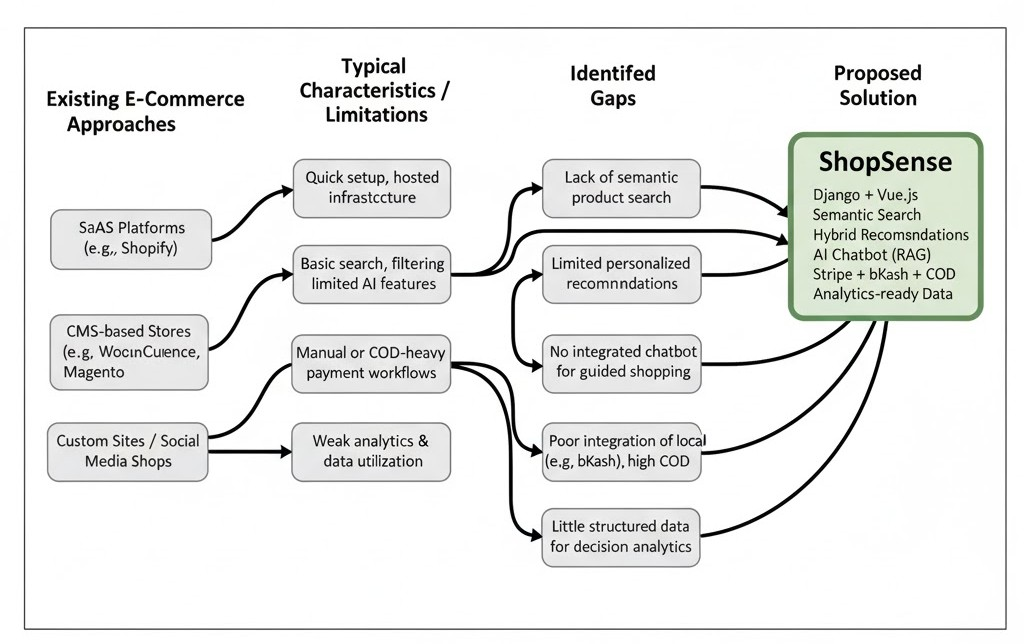
\includegraphics[width=0.9\textwidth]{Images/MyFigs/literature-gaps-overview.jpg}
  \caption{ShopSense targets the identified gaps and existing e-commerce platforms in this conceptual overview.}
  \label{fig:literature-gaps-overview}
\end{figure}

\section{Conclusion}
This chapter reviews existing e-commerce platforms, web frameworks, AI techniques for chatbots, semantic search, and recommendation systems, alongside online payment integrations relevant to the Bangladeshi context\cite{laudon2021ecommerce,holovaty2009django,adamopoulou2020chatbots,lewis2020retrieval,reimers2019sentence,ricci2015recommender,koren2009matrix,hasan2021mobile}. The analysis highlights several shortcomings of typical small and medium-sized online stores, such as limited intelligence in product discovery, insufficient personalization, fragmented customer support, incomplete payment integration, and weak analytics (summarized in Figure~\ref{fig:literature-gaps-overview}). 

These observations motivate the design of \textit{ShopSense}. \textit{ShopSense} aims to provide an integrated, AI-enhanced e-commerce platform with semantic search, recommendations, chat-bot assistance, and multi-gateway payment support. The next chapter presents the design methods and system architecture used to realize this platform.

